% ============================================================
% MAT670 -- Lectures 9 and 10 (source: MAT670_9X, pp. 1--29)
%   Lecture 9:  pp. 1--15
%   Lecture 10: pp. 16--29
% ============================================================
\chapter{Lecture 9: More on functions and their critical points}
\label{L9:chap}

Last time we defined a smooth function $f\colon M\to\R$ on a manifold $M$ to be
\emph{Morse} if it has no degenerate critical points.%
\fixed{notes say ``no non-degenerate critical points''}
\added{That is, every critical point of $f$ is non-degenerate.}

\section{What does this mean?}
\label{L9:sec:meaning}

To make sense of this definition we need to understand criticality, so we introduce
the tangent space $T_pM$ at a point $p\in M$.

\begin{center}
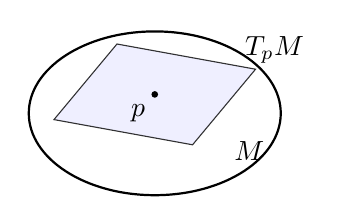
\begin{tikzpicture}[scale=0.8]
  \draw[thick] (0,0) ellipse (2 and 1.3);
  \node at (1.5,-0.6) {$M$};
  \draw[fill=blue!8,opacity=0.8] (-1.6,-0.1) -- (0.6,-0.5) -- (1.6,0.7) -- (-0.6,1.1) -- cycle;
  \fill (0,0.3) circle (1.5pt) node[below left] {$p$};
  \node at (1.9,1.0) {$T_pM$};
\end{tikzpicture}
\end{center}

We consider velocities of curves
\[
  \gamma\colon[-1,1]\to M,\qquad \gamma(0)=p,
\]
and, with respect to a chart $\varphi\colon U\to\R^n$ with $p\in U\subset M$, we ask
that $\varphi\circ\gamma\colon[-1,1]\to\R^n$ be differentiable at $0$.
The classes of such curves, where two curves are identified when their tangents
\added{$(\varphi\circ\gamma)'(0)$} at $0$ agree, define the \emph{tangent space} $T_pM$ at $p$.
\added{(This identification does not depend on the chart, since the transition maps
are diffeomorphisms; the tangent vector represented by $\gamma$ is written $\gamma'(0)$.)}

Given a smooth map $f\colon M\to N$, there is an induced \emph{linear} map
\[
  f_*\colon T_pM\to T_{f(p)}N,\qquad f_*\bigl(\gamma'(0)\bigr)=(f\circ\gamma)'(0),
\]
\fixed{notes: target $T_pN$}
called the \emph{differential} or \emph{push-forward} of $f$.

\begin{definition}
\label{L9:def:critical}
Let $f\colon M\to\R$ be smooth. A point $p\in M$ is a \emph{critical point} of $f$ if
\[
  f_*\colon T_pM\to T_{f(p)}\R
\]
is the zero map. The value $f(p)$ is then called a \emph{critical value}.
\end{definition}

In local coordinates $(x_1,\dots,x_n)$ \added{about $p$} this is written
\[
  \frac{\partial f}{\partial x_i}\Big|_p = 0\qquad\text{for all } i=1,\dots,n .
\]
Also, there is a bilinear form \added{on $T_pM$, well defined at a critical point $p$,} which can be
written similarly in coordinates as
\[
  H_f(p)=\Bigl(\frac{\partial^2 f}{\partial x_i\,\partial x_j}\Big|_p\Bigr)_{i,j},
  \qquad\text{also written } f_{**}(p).
\]
This is the \emph{Hessian} of $f$ at $p$.

\begin{definition}
\label{L9:def:nondeg}
A critical point $p$ of $f$ is \emph{non-degenerate} if the Hessian $H_f(p)$ is
non-degenerate, i.e.\ its matrix is non-singular. The \emph{index} of $f$ at $p$ is the
number of negative eigenvalues of $H_f(p)$ \added{(the dimension of a maximal subspace of
$T_pM$ on which $H_f(p)$ is negative definite)}.
\end{definition}

The notion of index is well defined in this case.
\added{Indeed, under a change of coordinates the Hessian at a critical point changes by
$H\mapsto J^{\mathsf T}HJ$ with $J$ the (invertible) Jacobian, and by Sylvester's law of inertia the number
of negative eigenvalues is unchanged.}

\section{Why do we care about non-degenerate critical points?}
\label{L9:sec:morselemma}
\orig{numbered 6.2--6.4 in the notes; read as 9.2--9.4}

\begin{lemma}[Morse Lemma]
\label{L9:lem:morse}
If $p$ is a non-degenerate critical point of a smooth function $f$, there is a local
coordinate system $(x_1,\dots,x_n)$ about $p$ \added{with $p$ at the origin} such that
\[
  f = \added{f(p)}\ - \sum_{i=1}^{\lambda} x_i^2 + \sum_{j=\lambda+1}^{n} x_j^2 ,
\]
where $\lambda$ is the index of $f$ at $p$.
\end{lemma}

\begin{proof}[Proof (sketch)]
We may shift so that $f(p)=0$ \added{and $p=0$ in some chart}. By the fundamental theorem of
calculus and the integral form of Taylor's theorem,
\[
  f(x_1,\dots,x_n)=\int_0^1 \frac{d}{dt}f(tx)\,dt
  =\int_0^1\sum_{i=1}^n \frac{\partial f}{\partial x_i}(tx_1,\dots,tx_n)\,x_i\,dt ,
\]
\added{so $f=\sum_i x_i g_i$ with $g_i$ smooth and $g_i(0)=\frac{\partial f}{\partial x_i}(0)=0$.
Applying the same argument to each $g_i$,}
and in fact
\[
  f(x_1,\dots,x_n)=\sum_{i,j} h_{ij}(x_1,\dots,x_n)\,x_ix_j
\]
for some smooth functions $h_{ij}$. We can symmetrize ($h_{ij}=h_{ji}$, replacing $h_{ij}$
by $\tfrac12(h_{ij}+h_{ji})$) and compute
\[
  h_{ij}(0)=\frac12\,\frac{\partial^2 f}{\partial x_i\,\partial x_j}(0)
\]
\fixed{notes: $\partial f$ for $\partial^2 f$}
in some coordinate system for $T_pM$.
This can be inductively diagonalized in a neighbourhood of $p$, for example via the
spectral theorem plus a continuity argument.

\emph{Example in dimension 2.} Write
\[
  f(x,y)=x^2h_{11}+2xy\,h_{12}+y^2h_{22},
  \qquad \frac{\partial^2 f}{\partial x^2}\Big|_{(0,0)}=2h_{11}(0,0),\ \text{etc.}
\]
By a \added{linear} coordinate change we may assume $h_{11}(0,0)\neq0$; by continuity there is
a neighbourhood on which $h_{11}\neq0$. Then we can define a local change of coordinates
\[
  \bar x=\sqrt{\abs{h_{11}}}\Bigl(x+\frac{h_{12}}{h_{11}}\,y\Bigr)
  \quad\Longrightarrow\quad
  \bar x^2=\abs{h_{11}}\Bigl(x^2+2\frac{h_{12}}{h_{11}}xy+\frac{h_{12}^2}{h_{11}^2}y^2\Bigr).
\]
In the case $h_{11}>0$,
\[
  \bar x^2=h_{11}x^2+2h_{12}xy+\frac{h_{12}^2}{h_{11}}y^2 ,
\]
and since
\[
  f=\underbrace{x^2h_{11}+2xy\,h_{12}}_{=\ \bar x^2-\frac{h_{12}^2}{h_{11}}y^2}+\,y^2h_{22},
  \qquad\text{we get}\qquad
  f=\bar x^2+\Bigl(h_{22}-\frac{h_{12}^2}{h_{11}}\Bigr)y^2 .
\]
\added{Non-degeneracy at $0$ means $h_{11}h_{22}-h_{12}^2\neq0$ there, so the coefficient of $y^2$
is non-zero near $0$, and $\bar y=\sqrt{\abs{h_{22}-h_{12}^2/h_{11}}}\;y$ finishes the job.
(The Jacobian of $(x,y)\mapsto(\bar x,\bar y)$ at $0$ is invertible, so this is a coordinate
change by the inverse function theorem.)}
The proof proceeds the same way for the other cases and for higher dimensions.
\begin{addedblock}
In general, after a linear change we have $h_{11}(0)\ne0$; put
$\bar x_1=\sqrt{\abs{h_{11}}}\,\bigl(x_1+\sum_{j>1}x_jh_{1j}/h_{11}\bigr)$, so that
$f=\pm\bar x_1^2+\sum_{i,j\ge2}x_ix_j\,h'_{ij}$ with $h'_{ij}$ smooth and symmetric and
$(h'_{ij}(0))$ non-singular; induct on $n$. (See Milnor, \emph{Morse Theory}, Lemma 2.2.)
\end{addedblock}
\end{proof}

\begin{corollary}
\label{L9:cor:isolated}
Non-degenerate critical points are isolated.
\end{corollary}
\begin{addedblock}
Indeed, in Morse coordinates $df=(-2x_1,\dots,-2x_\lambda,2x_{\lambda+1},\dots,2x_n)$ vanishes
only at the origin.
\end{addedblock}

\section{One-parameter groups of diffeomorphisms}
\label{L9:sec:oneparam}

\begin{definition}
\label{L9:def:oneparam}
A \emph{one-parameter group of diffeomorphisms} of a manifold $M$ is a smooth map
\[
  \Phi\colon\R\times M\to M
\]
such that
\begin{enumerate}[nosep]
  \item for each $t\in\R$, the map $\varphi_t\colon M\to M$ defined as
        $\varphi_t(p)=\Phi(t,p)$ is a diffeomorphism of $M$ onto $M$, and
  \item for all $t,s\in\R$, $\varphi_{t+s}=\varphi_t\circ\varphi_s$.
\end{enumerate}
\end{definition}
\orig{$\Phi$ vs.\ $\varphi_t$ distinction added in blue on the page}

This defines a vector field $X$ on $M$: for a smooth $f\colon M\to\R$, $X$ is characterized by
\[
  X_q(f)=\lim_{h\to0}\frac{f(\varphi_h(q))-f(q)}{h}.
\]
So this is an assignment of a direction to each point $q$ of $M$, and $X_q$ takes a
directional derivative of $f$. We say that $X$ \emph{generates} the group $\varphi$.

\begin{lemma}
\label{L9:lem:flow}
A smooth vector field on $M$ which vanishes outside of a compact set $K\subset M$ generates
a unique one-parameter group of diffeomorphisms of $M$.
\end{lemma}

\begin{proof}
Consider a smooth curve $\gamma\colon t\mapsto\gamma(t)\in M$ with velocity vector
$\frac{d\gamma}{dt}\in T_{\gamma(t)}M$, characterized by
\[
  \frac{d\gamma}{dt}f=\lim_{h\to0}\frac{f(\gamma(t+h))-f(\gamma(t))}{h}.
\]
Let $\varphi$ be a one-parameter group of diffeomorphisms generated by a vector field $X$ as in
the lemma. Then for fixed $q$, the curve $t\mapsto\varphi_t(q)$ satisfies
\begin{equation}\label{L9:eq:ode}
  \frac{d\varphi_t(q)}{dt}=X_{\varphi_t(q)},\qquad \varphi_0(q)=q ,
\end{equation}
since
\[
  \frac{d\varphi_t(q)}{dt}(f)=\lim_{h\to0}\frac{f(\varphi_{t+h}(q))-f(\varphi_t(q))}{h}
  =\lim_{h\to0}\frac{f\bigl(\varphi_h(\varphi_t(q))\bigr)-f(\varphi_t(q))}{h}
  =X_{\varphi_t(q)}(f).
\]
\added{This already gives uniqueness: any group generated by $X$ consists of solutions of
\eqref{L9:eq:ode}, which are unique.}

\emph{Existence.} By existence and uniqueness of solutions of ODEs (Picard--Lindel\"of, applied in
local coordinates), the system \eqref{L9:eq:ode} has a unique solution that depends smoothly on
the initial conditions. Hence for every $q\in M$ there is a neighbourhood $U$ of $q$ and
an $\varepsilon>0$ such that \eqref{L9:eq:ode} has a unique smooth solution for initial points in
$U$ and $\abs{t}<\varepsilon$.

Since $K$ is compact, \added{finitely many such neighbourhoods cover $K$, so} there is a minimal
$\varepsilon>0$ for such a cover of $K$. For $q\notin K$, let $\varphi_t(q)=q$
\added{(this solves \eqref{L9:eq:ode} since $X$ vanishes there)}. Hence there is a unique smooth
solution $\varphi_t(q)$, $\abs{t}<\varepsilon$, for all $q\in M$.
Note that
\[
  \varphi_{t+s}=\varphi_t\circ\varphi_s\qquad\text{for }\abs{t},\abs{s},\abs{t+s}<\varepsilon
\]
\added{(both sides solve \eqref{L9:eq:ode} in $t$ with the same initial value $\varphi_s(q)$)}.
So $\varphi_t$ is a diffeomorphism for $\abs{t}<\varepsilon$ \added{with inverse $\varphi_{-t}$}.

But we can iterate this process for $t\ge\varepsilon$:
\unclear{``by LNP\dots''; step size $\varepsilon$ vs.\ $\varepsilon/2$ unclear}
writing $t=k\,\tfrac{\varepsilon}{2}+r$ with $k=\lfloor 2t/\varepsilon\rfloor$ and
$0\le r<\tfrac{\varepsilon}{2}$, \added{define
$\varphi_t=\varphi_{\varepsilon/2}\circ\cdots\circ\varphi_{\varepsilon/2}\circ\varphi_r$ ($k$ factors),
and $\varphi_{-t}=(\varphi_t)^{-1}$. One checks that this is well defined, smooth, and satisfies the group law.}
\end{proof}

\section{The diffeomorphism theorem}
\label{L9:sec:diffeo}
\orig{title ``Homotopy Theorem'' crossed out, replaced by ``Diffeomorphism''}

For $f\colon M\to\R$ we have the \emph{sublevel sets}
\[
  M^a:=f^{-1}(-\infty,a]=\{p\in M: f(p)\le a\}.
\]
\orig{notes mix $M_a$ and $M^a$}

\begin{theorem}
\label{L9:thm:diffeo}
Let $f\colon M\to\R$ be a smooth function, let $a<b$, and suppose $f^{-1}[a,b]$ is compact and
contains no critical points of $f$. Then $M^a$ is diffeomorphic to $M^b$.
\added{Moreover, $M^a$ is a deformation retract of $M^b$.}
\end{theorem}

\emph{Idea.} Push $f^{-1}(b)$ down to $f^{-1}(a)$ along $-\nabla f$.

\begin{center}
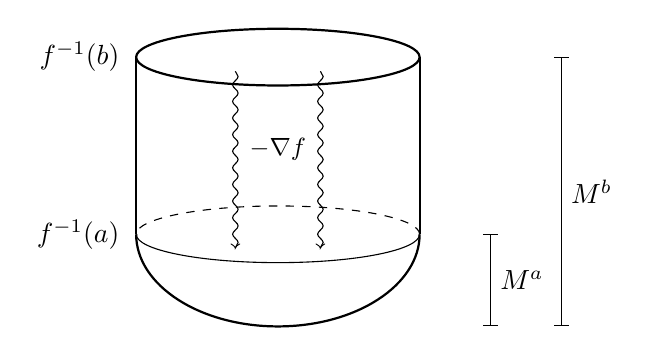
\begin{tikzpicture}[scale=0.9]
  % lower cap region M^a
  \draw[thick] (-2,0) arc (180:360:2 and 1.3);
  \draw[thick] (-2,0) -- (-2,2.5);
  \draw[thick] (2,0) -- (2,2.5);
  \draw[thick] (0,2.5) ellipse (2 and 0.4);
  \draw (-2,0) arc (180:360:2 and 0.4);
  \draw[dashed] (2,0) arc (0:180:2 and 0.4);
  \draw[->,decorate,decoration={snake,amplitude=1pt,segment length=6pt}] (-0.6,2.3) -- (-0.6,-0.2);
  \draw[->,decorate,decoration={snake,amplitude=1pt,segment length=6pt}] (0.6,2.3) -- (0.6,-0.2);
  \node[left] at (-2.1,2.5) {$f^{-1}(b)$};
  \node[left] at (-2.1,0) {$f^{-1}(a)$};
  \node at (0,1.2) {\small $-\nabla f$};
  \draw[|-|] (3,-1.3) -- (3,0) node[midway,right] {$M^a$};
  \draw[|-|] (4,-1.3) -- (4,2.5) node[midway,right] {$M^b$};
\end{tikzpicture}
\end{center}

\begin{proof}
$M$ admits a \added{Riemannian} metric; we need it to define $\langle X,Y\rangle$, the inner product
of tangent vectors. So we can define the gradient $\nabla f$, which is the vector field
characterized by
\[
  \langle X,\nabla f\rangle = Xf
\]
for any vector field $X$; that is, $\langle X,\nabla f\rangle$ is the directional derivative of $f$
along $X$. Note that $\nabla f$ vanishes exactly at the critical points of $f$.
If $\gamma\colon\R\to M$ is a curve with velocity vector $\frac{d\gamma}{dt}$, then
\fixed{notes: $\gamma\colon\R\to\R$}
\[
  \Bigl\langle\frac{d\gamma}{dt},\nabla f\Bigr\rangle=\frac{d(f\circ\gamma)}{dt}.
\]

Define a smooth function $\rho\colon M\to\R$ that is
\[
  \rho=\frac{1}{\langle\nabla f,\nabla f\rangle}\quad\text{on } f^{-1}[a,b],
\]
and $0$ outside of a compact neighbourhood of $f^{-1}[a,b]$
\added{(chosen to contain no critical points, which is possible since the critical set is closed
and $f^{-1}[a,b]$ is compact)}.
Then the vector field $X$ defined as
\[
  X_q=\rho(q)\,(\nabla f)_q
\]
satisfies the hypotheses of Lemma~\ref{L9:lem:flow} (it is smooth and vanishes outside a compact
set), so there is a one-parameter group of diffeomorphisms $\varphi_t\colon M\to M$ generated by $X$.

For fixed $q$, consider $t\mapsto f(\varphi_t(q))$. If $\varphi_t(q)\in f^{-1}[a,b]$, then
\[
  \frac{d f(\varphi_t(q))}{dt}=\Bigl\langle\frac{d\varphi_t(q)}{dt},\nabla f\Bigr\rangle
  =\langle X,\nabla f\rangle = 1 .
\]
So $t\mapsto f(\varphi_t(q))$ is linear with derivative $1$ while $f(\varphi_t(q))$ lies in $[a,b]$.
Therefore $\varphi_{b-a}\colon M\to M$ is a diffeomorphism which carries $M^a$
\added{onto} $M^b$.

\begin{center}
\begin{tikzpicture}[scale=0.8]
  \draw[thick] (-1.5,0) -- (-1.5,3); \draw[thick] (1.5,0) -- (1.5,3);
  \draw[thick] (0,3) ellipse (1.5 and 0.3);
  \draw (0,1.5) ellipse (1.5 and 0.3);
  \draw[thick] (-1.5,0) arc (180:360:1.5 and 0.3);
  \draw[dashed] (1.5,0) arc (0:180:1.5 and 0.3);
  \draw[-{Latex}] (0,-0.3) -- (0,1.2); \draw[-{Latex}] (0,1.2) -- (0,2.7);
  \fill (0,-0.3) circle (1.5pt);
  \node[right] at (1.6,3) {$f=b$}; \node[right] at (1.6,0) {$f=a$};
  \node[left] at (-1.6,1.5) {$\varphi_t$};
  \node at (4.2,1.5) {\small $\varphi_{b-a}\colon M^a\xrightarrow{\ \cong\ }M^b$};
\end{tikzpicture}
\end{center}
\orig{p.\,15: sketch of this flow}

Furthermore, define $r_t\colon M^b\to M^b$, $0\le t\le 1$, by
\fixed{notes: $r_t\colon M_b\to M_a$}
\[
  r_t(q)=\begin{cases}
    q & \text{if } f(q)\le a,\\
    \varphi_{t(a-f(q))}(q) & \text{if } a\le f(q)\le b.
  \end{cases}
\]
Then $r_0=\mathrm{id}$, and $r_1$ is a retraction from $M^b$ to $M^a$; \added{$r_t$ is continuous
since the two formulas agree on $f^{-1}(a)$.} Hence $r_t$ is a deformation retraction
\added{of $M^b$ onto $M^a$.}
\added{(Cf.\ Milnor, \emph{Morse Theory}, Theorem 3.1.)}
\end{proof}

% ============================================================
\chapter{Lecture 10: Configuration spaces and Morse-like results}
\label{L10:chap}
\orig{p.\,16, boxed: ``need to be rewritten, out of order / missing pieces''}

\section{Recap and the handle attachment theorem}
\label{L10:sec:recap}

For smooth functions we have the diffeomorphism result (Theorem~\ref{L9:thm:diffeo}) that says:
if $f\colon M\to\R$, $a<b$, $f^{-1}[a,b]$ is compact, and there are no critical values in $[a,b]$,
then $M^a$ is diffeomorphic to $M^b$.

There is also a handle attachment theorem (not proved here) for smooth $f\colon M\to\R$:

\begin{theorem}[Handle attachment]
\label{L10:thm:handle}
Let $p$ be a non-degenerate critical point of $f$ with index $\lambda$ and $f(p)=c$.
Suppose there is $\varepsilon>0$ such that $f^{-1}[c-\varepsilon,c+\varepsilon]$ is compact and
contains no critical points other than $p$. Then $M^{c+\varepsilon}$ has the homotopy type of
$M^{c-\varepsilon}\cup_g e^\lambda$, \added{that is, $M^{c-\varepsilon}$ with a $\lambda$-cell attached
along a map $g\colon\partial e^\lambda\to M^{c-\varepsilon}$}.
\end{theorem}
\added{(Milnor, \emph{Morse Theory}, Theorem 3.2.)}

\subsection*{Morse-type inequalities}
Let $c_\lambda$ be the number of critical points of index $\lambda$ \added{of a Morse function on a
compact manifold $M$}. The homotopy type changes by attaching various cells of index $\lambda$ as we
``climb'' $M$ via the Morse function. Consequently
\[
  \sum_\lambda(-1)^\lambda c_\lambda=\chi(M),
\]
and in general we have the constraints
\[
  c_\lambda\ \ge\ b_\lambda(M),
\]
where $b_\lambda(M)$ is the $\lambda$-th Betti number of $M$ (the rank of the $\lambda$-th homology group).
\added{(These are the weak Morse inequalities.)}
The key point for us is that the Betti numbers can be computed for many spaces we like.

\section{Betti numbers for the configuration space of points on \texorpdfstring{$\Sph^2$}{S2}}
\label{L10:sec:betti}

Let $B\Conf(N)$ denote the configuration space of $N$ points on $\Sph^2$
\added{modulo rotations, $B\Conf(N)=\Conf(N,\Sph^2)/\SO(3)$.}
\unclear{meaning of ``$B$'' not on page; quotient by $\SO(3)$ inferred}
Via stereographic projection \added{from the first point}, for $N\ge3$ we have a
\added{diffeomorphism}
\[
  B\Conf(N)\ \xrightarrow{\ \cong\ }\ \Conf(N-1,\R^2)/\SO(2).
\]
\begin{addedblock}
Indeed, $\SO(3)$ acts transitively on $\Sph^2$, so we may rotate $u_1$ to the north pole; the
remaining freedom is the stabilizer $\SO(2)$ of the pole, and stereographic projection from the
pole identifies $\Sph^2\setminus\{u_1\}$ with $\R^2$, $\SO(2)$-equivariantly (rotations about the
origin). For $N\ge3$ the actions are free.
\end{addedblock}
That allows us to compute Betti numbers from known Betti numbers \added{via the
fibration $\SO(2)\to\Conf(N-1,\R^2)\to\Conf(N-1,\R^2)/\SO(2)$}: the Poincar\'e polynomial is
\[
  P\bigl(B\Conf(N)\bigr)=\frac{P\bigl(\Conf(N-1,\R^2)\bigr)}{P(\SO(2))},
\]
where
\[
  P\bigl(\Conf(N-1,\R^2)\bigr)=(1+t)(1+2t)\cdots\bigl(1+(N-2)t\bigr),\qquad P(\SO(2))=1+t .
\]
\begin{addedblock}
Here $P(X)(t)=\sum_i b_i(X)\,t^i$. The formula for $\Conf(n,\R^2)$ is due to Arnold (1969). The
division is justified because the $\SO(2)$-bundle is trivial: the map
$u\mapsto (u_2-u_1)/\abs{u_2-u_1}\in \Sph^1$ is $\SO(2)$-equivariant, so
$\Conf(N-1,\R^2)\cong \SO(2)\times\bigl(\Conf(N-1,\R^2)/\SO(2)\bigr)$, and the K\"unneth formula
applies. Hence
\[
  P\bigl(B\Conf(N)\bigr)=(1+2t)(1+3t)\cdots\bigl(1+(N-2)t\bigr).
\]
\end{addedblock}

The picture behind the formula for $\Conf(n,\R^2)$ is that of punctured planes, and the induction
up \added{in $n$: forgetting the last point gives a fibration
$\Conf(n,\R^2)\to\Conf(n-1,\R^2)$ whose fibre is the plane with $n-1$ punctures, with Poincar\'e
polynomial $1+(n-1)t$ (Fadell--Neuwirth)}.

So the Betti numbers $b_\lambda$ of $B\Conf(N)$ are:
\begin{center}
\begin{tabular}{c|cccc}
\toprule
 & $\lambda=0$ & $\lambda=1$ & $\lambda=2$ & $\lambda=3$ \\
\midrule
$N=3$ & $1$ & $0$ & $0$ & $0$\\
$N=4$ & $1$ & $2$ & $0$ & $0$\\
$N=5$ & $1$ & $5$ & $6$ & $0$\\
\added{$N=6$} & \added{$1$} & \added{$9$} & \added{$26$} & \added{$24$}\\
$\vdots$ & $1$ & & & \\
\bottomrule
\end{tabular}
\end{center}
In general $b_0=1$, and the top Betti number is $b_{N-3}=(N-2)!$.

One can use this idea to describe extensions and induction arguments for configuration spaces in
general; for example the $K(\pi,1)$ type of configuration spaces comes from the fact that such spaces
really change nicely \added{(the Fadell--Neuwirth fibrations: inductively, $\Conf(n,\R^2)$ is an
iterated fibration with aspherical fibres, so it is aspherical, with fundamental group the pure
braid group $P_n$)}.
\orig{some crossed-out words here}

\section{Min-type functions}
\label{L10:sec:mintype}
\orig{numbered 10.2 again in the notes}

\begin{definition}
\label{L10:def:mintype}
A \emph{min-type function} is given by a parametrized family of functions
\[
  f(x,p)\colon X\times M\to\R ,
\]
where $X$ is a parameter space, compact\dots; for our purposes, finite and discrete. We require
$f(x,\cdot)$ to be smooth (or smooth enough) for each parameter $x$. The min-type function is then
\[
  F(p)=\added{\min_{x\in X}f(x,p).}
\]
\end{definition}

Our function, the injectivity radius
\[
  \rho\colon\Conf(N)\to\R,\qquad \rho(u)=\min_{\substack{i\ne j\\ u_i,u_j\in u}} d(u_i,u_j),
\]
is of this type \added{(with $X$ the set of pairs $\{i,j\}$ and $f(\{i,j\},u)=d(u_i,u_j)$, the
geodesic distance on $\Sph^2$)}.
\added{(Here ``injectivity radius'' means the minimal distance; the largest radius of disjoint
spherical caps centred at the $u_i$ is $\rho(u)/2$.)}

In general, topological regularity is characterized by the non-emptiness of an intersection of
gradient cones of this type.
\begin{addedblock}
Precisely: for $p\in M$ let $X(p)=\{x\in X: f(x,p)=F(p)\}$ be the active parameters, and let
\[
  C_p=\{v\in T_pM:\ df_x|_p(v)>0\ \text{for all } x\in X(p)\}
\]
be the cone of directions that increase every active function, hence increase $F$ to first order.
Where $C_p\ne\emptyset$, a gradient-like vector field can be built locally, and the flow argument of
Theorem~\ref{L9:thm:diffeo} goes through for superlevel sets $\{F\ge c\}$
(cf.\ Baryshnikov--Bubenik--Kahle, \emph{Min-type Morse theory for configuration spaces of hard
spheres}, IMRN 2014).
\end{addedblock}

\begin{corollary}
\label{L10:cor:topchange}
The topology \added{of the superlevel sets of $F$} only changes at critical points $x$, which only
occur when the gradient cone is empty, i.e.\ when
\[
  \sum_{x} w_x\,df_x\big|_u=0\qquad\text{for some } w_x\ge0 \added{\text{ not all zero, } x\in X(u)}.
\]
\end{corollary}
\added{The equivalence of ``$C_u=\emptyset$'' and the existence of such weights is Gordan's theorem
of the alternative (a finite-dimensional Farkas/separation lemma).}

From our picture for the injectivity radius, this is when increasing some collection
\added{of active distances simultaneously} is not possible.
\unclear{p.\,21 right column only partly legible}

\begin{center}
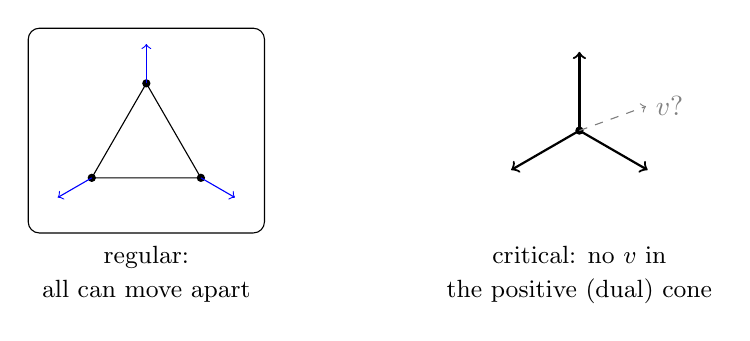
\begin{tikzpicture}[scale=1]
  % regular: three points in a box, can all move apart
  \begin{scope}
    \draw[rounded corners] (-1.5,-1.1) rectangle (1.5,1.5);
    \coordinate (A) at (90:0.8); \coordinate (B) at (210:0.8); \coordinate (C) at (330:0.8);
    \draw (A) -- (B) -- (C) -- cycle;
    \foreach \P/\a in {A/90,B/210,C/330} { \fill (\P) circle (1.5pt); \draw[->,blue] (\P) -- ++(\a:0.5); }
    \node[below,align=center] at (0,-1.15) {\small regular:\\ \small all can move apart};
  \end{scope}
  % critical: three gradient directions at 120 degrees
  \begin{scope}[xshift=5.5cm,yshift=0.2cm]
    \fill (0,0) circle (1.5pt);
    \foreach \a in {90,210,330} \draw[->,thick] (0,0) -- (\a:1);
    \draw[->,dashed,gray] (0,0) -- (20:0.9) node[right] {$v$?};
    \node[below,align=center] at (0,-1.35) {\small critical: no $v$ in\\ \small the positive (dual) cone};
  \end{scope}
\end{tikzpicture}
\end{center}

\subsection{The contact graph and balanced configurations}
\orig{p.\,22 left column crossed out}

Let $u\in\Conf(N)$ with $\rho(u)\ge\theta$ \added{(we will take $\rho(u)=\theta$)}. There is a
\emph{contact graph}:
\begin{itemize}[nosep]
  \item vertices: the points $u_i\in u$;
  \item edges: $u_iu_j$ whenever $d(u_i,u_j)=\theta$.
\end{itemize}
Edges may be assigned positive weights $w_{ij}$, and if the resulting weighted graph is
\emph{force balanced}, this is equivalent to the cone being empty.
\begin{addedblock}
Write $e_{ij}\in T_{u_i}\Sph^2$ for the unit tangent vector at $u_i$ pointing along the geodesic
towards $u_j$. The differential of $d(u_i,u_j)$ has component $-e_{ij}$ at $u_i$ and $-e_{ji}$ at
$u_j$. So the condition of Corollary~\ref{L10:cor:topchange} reads: there are weights $w_{ij}\ge0$,
not all zero, on the edges of the contact graph with
\[
  \sum_{j\sim i} w_{ij}\,e_{ij}=0\qquad\text{at every vertex } u_i ,
\]
i.e.\ the ``forces'' along the edges balance at each point. The edges with $w_{ij}>0$ form the
\emph{balanced (stressed) subgraph}.
\end{addedblock}

So the only obstacles to topological regularity are exactly the force balanced configurations of
points.

\emph{Examples\dots}
\orig{left blank on p.\,23}

\begin{definition}
\label{L10:def:conftheta}
\added{$\Conf(N,\theta)=\{u\in\Conf(N,\Sph^2):\rho(u)\ge\theta\}$, and $\Conf(N,0):=\Conf(N,\Sph^2)$.}
\end{definition}

\begin{theorem}
\label{L10:thm:smalltheta}
Suppose $N\ge3$.
\unclear{``$N\ge3$'' or ``$N>3$''}
Then for $0<\theta<\pi/N$, $\Conf(N,\theta)$ is a strong deformation retract of, and hence homotopy
equivalent to, $\Conf(N,0)$.
\end{theorem}

\begin{proof}[Proof (sketch)]
First, there are no balanced configurations \added{with $\rho(u)=\theta'$ for $0<\theta'<\pi/N$};
then push each point apart \added{using the flow of a gradient-like vector field for $\rho$}\dots
\begin{addedblock}
\emph{No balanced configurations.} (i) A balanced subgraph is not contained in any open hemisphere:
if all its vertices lie in $\{y:\langle y,e\rangle>0\}$, take a vertex $v$ of the subgraph minimizing
$\langle v,e\rangle$. For each neighbour $u$, the vector $e_{vu}$ is a positive multiple of
$u-\langle u,v\rangle v$, whose $e$-component is $\langle u,e\rangle-\langle u,v\rangle\langle v,e\rangle
\ge\langle v,e\rangle(1-\langle u,v\rangle)>0$ (using $\langle u,e\rangle\ge\langle v,e\rangle$ and $\langle u,v\rangle<1$). So every force at $v$ has a positive $e$-component,
and they cannot sum to zero.
(ii) Each connected component of the balanced subgraph is itself balanced. If a component has $k$
vertices, a spanning tree has $k-1$ edges of length $\theta'$, total length $L=(k-1)\theta'$. A tree
has a centre $c$ within distance $L/2$ (along the tree) of all its points, so all vertices lie in the
spherical ball of radius $L/2$ about $c$. By (i), $L/2\ge\pi/2$, so $(k-1)\theta'\ge\pi$, so
$\theta'\ge\pi/(k-1)\ge\pi/(N-1)>\pi/N$.
(So this crude argument even gives the theorem for $\theta<\pi/(N-1)$. The sharp bound is
$\theta<2\pi/N$: a balanced graph has every valence $\ge2$, hence at least as many edges as
vertices, and Kusner--Kusner--Lagarias--Shlosman (Thm.~4.14, cited below) show its total length is at least
$2\pi$, with equality only for the $N$ points equally spaced on a great circle. Compare the
statement at the start of Lecture~11.)

\emph{Deformation.} So $\rho$ has no critical values in $(0,\theta]$, and the min-type version of
Theorem~\ref{L9:thm:diffeo} lets us push $\{\rho\ge\eta\}$ onto $\{\rho\ge\theta\}$ for every
$0<\eta<\theta$; some care is needed near $\rho=0$, where $\Conf(N,0)$ is not compact. (Cf.\
Kusner--Kusner--Lagarias--Shlosman, \emph{Configuration spaces of equal spheres touching a given
sphere: the twelve spheres problem}, arXiv:1611.10297 (2016); in \emph{New Trends in Intuitive
Geometry}, Bolyai Soc.\ Math.\ Stud.\ 27, Springer, 2018.)
\end{addedblock}
\end{proof}

For $N=4$ \dots, $\Conf(N,\theta)$ for small $\theta$ is therefore path connected.
\unclear{``$N=4$'' or ``$N>4$''}
\added{(Indeed $\Conf(N,\Sph^2)$ is connected, since the diagonals removed have real codimension~2.)}

\begin{example}[$N=4$]
\label{L10:ex:N4}
\orig{left blank in the notes}
\added{Balanced subgraphs need every vertex of valence $\ge2$, and a vertex of valence $2$ must have
its two edges in opposite directions, so it lies on a great circle through its two neighbours. One
finds: the square on a great circle ($\theta=\pi/2$), and the regular tetrahedron
($\theta=\arccos(-1/3)\approx109.47^\circ$, the maximum of $\rho$). An equilateral triangle on a great
circle ($\theta=2\pi/3$) plus a free fourth point is \emph{not} realizable, since every point of
$\Sph^2$ is within $\pi/2$ of one of the three. This is the editor's check; compare the question marks on p.\,29.}
\end{example}

\subsection{Outlook}
\orig{pp.\,24--25: headings only}
\begin{itemize}[nosep]
  \item Strata for Tammes maxima: table\dots
  \added{(The Tammes problem asks for $\max\rho$ over $\Conf(N,\Sph^2)$; it is solved for
  $N\le14$ and $N=24$, with $N=13,14$ due to Musin--Tarasov, 2012/2015.)}
  \item An algorithm for searching \added{for critical configurations} by evolution of force
  configurations\dots
  \item Local maxima; rings\dots
  \item Rigidity?, critical conditions and weights\dots
  \item Candidate graph sorting\dots
\end{itemize}

\section{Topological regularity revisited}
\label{L10:sec:revisit}
\orig{pp.\,26--29 seem to re-explain \S\ref{L10:sec:mintype}; possibly a later lecture}

What is this? This is a force balanced \added{configuration}.
\unclear{p.\,26 has only these two lines}

That is, for the injectivity radius, \added{the gradient cone} is the intersection of the convex
cones of motions that increase the distance between each \added{active} pair of points.

\emph{Picture: three points.} The configuration space of $3$ points on $\Sph^2$ is $6$-dimensional.
Fixing one point leaves a $4$-dimensional space; fixing also the rotation angle $\psi$ about it
leaves a $3$-dimensional space, which is \added{locally} parametrized by the distances
$d_{12},d_{13},d_{23}$. The cone for $d_{12}$ is the upper half space $\{d_{12}\text{ increasing}\}$,
etc.
\orig{angle called $\theta$ in the notes}

\begin{center}
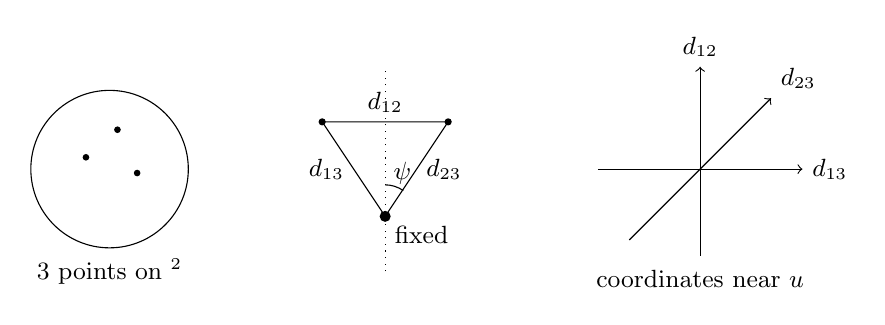
\begin{tikzpicture}[scale=1]
  \begin{scope}
    \draw (0,0) circle (1);
    \fill (-0.3,0.15) circle (1.2pt); \fill (0.35,-0.05) circle (1.2pt); \fill (0.1,0.5) circle (1.2pt);
    \node at (0,-1.3) {\small 3 points on $\Sph^2$};
  \end{scope}
  \begin{scope}[xshift=3.5cm]
    \draw[dotted] (0,-1.3) -- (0,1.3);
    \coordinate (P3) at (0,-0.6); \coordinate (P1) at (-0.8,0.6); \coordinate (P2) at (0.8,0.6);
    \draw (P1) -- node[above]{\small $d_{12}$} (P2) -- node[right]{\small $d_{23}$} (P3)
          -- node[left]{\small $d_{13}$} cycle;
    \fill (P1) circle (1.3pt); \fill (P2) circle (1.3pt); \fill (P3) circle (2pt);
    \node[below right] at (P3) {\small fixed};
    \draw (0,-0.2) arc (90:55:0.4); \node at (0.22,-0.05) {\small $\psi$};
  \end{scope}
  \begin{scope}[xshift=7.5cm]
    \draw[->] (-1.3,0) -- (1.3,0) node[right]{\small $d_{13}$};
    \draw[->] (0,-1.1) -- (0,1.3) node[above]{\small $d_{12}$};
    \draw[->] (-0.9,-0.9) -- (0.9,0.9) node[above right]{\small $d_{23}$};
    \node at (0,-1.4) {\small coordinates near $u$};
  \end{scope}
\end{tikzpicture}
\end{center}
\added{When the three active differentials are linearly independent, the three half-spaces meet in
an open octant, so the cone is non-empty and the value is regular.}

So:
\[
  \text{$\theta$ is a topologically regular value}\iff
  \begin{minipage}[c]{0.5\linewidth}
  neighbourhoods of the value have superlevel sets that deformation retract to each other.
  \end{minipage}
\]
\added{(For $\theta'<\theta$ near $\theta$, $\{\rho\ge\theta\}\hookrightarrow\{\rho\ge\theta'\}$ is
a deformation retract.)} So critical values are where the topology changes\dots

For topologically regular values, this deformation retraction is defined by the flow of some vector
field defined by $f$, the gradient flow as in the last lecture (Theorem~\ref{L9:thm:diffeo}).
So the topology can only change at an obstruction to gradient flow.
For a min-type function, this obstruction is given by a convex cone, namely the intersection
of all variational cones that increase $f$ at the parameters $x\in X$.

\begin{exercise}
\label{L10:ex:classify}
Classify all distinct realizable balanced configurations of $N$ points on a sphere.
\end{exercise}

First, list the graphs. For $3$ points, the candidate contact graphs are:
\begin{center}
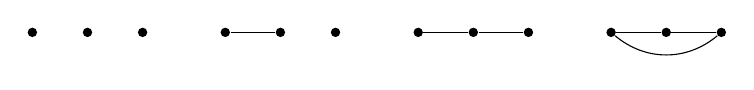
\begin{tikzpicture}[scale=0.7,every node/.style={circle,fill,inner sep=1.2pt}]
  \begin{scope}
    \node (a) at (0,0) {}; \node (b) at (1,0) {}; \node (c) at (2,0) {};
  \end{scope}
  \begin{scope}[xshift=3.5cm]
    \node (a) at (0,0) {}; \node (b) at (1,0) {}; \node (c) at (2,0) {}; \draw (a)--(b);
  \end{scope}
  \begin{scope}[xshift=7cm]
    \node (a) at (0,0) {}; \node (b) at (1,0) {}; \node (c) at (2,0) {}; \draw (a)--(b)--(c);
  \end{scope}
  \begin{scope}[xshift=10.5cm]
    \node (a) at (0,0) {}; \node (b) at (1,0) {}; \node (c) at (2,0) {}; \draw (a)--(b)--(c);
    \draw (a) to[bend right=40] (c);
  \end{scope}
\end{tikzpicture}
\end{center}
For example, to be force balanced every vertex needs valence $\ge2$
\unclear{reads ``valence $=2$''}
\added{(and a vertex of valence $2$ needs its two edges opposite, i.e.\ along a great circle). For
$N=3$ only the triangle survives, realized as three points at mutual distance $2\pi/3$ on a great
circle.}

Some graphs on $4$ points:
\begin{center}
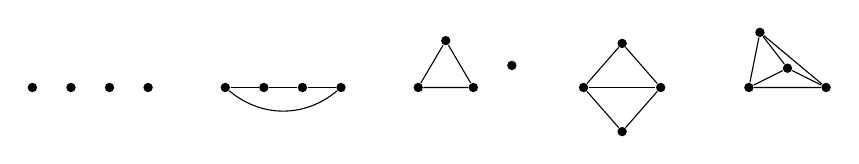
\begin{tikzpicture}[scale=0.7,every node/.style={circle,fill,inner sep=1.2pt}]
  \begin{scope}
    \foreach \i in {0,1,2,3} \node (p\i) at (\i*0.7,0) {};
  \end{scope}
  \begin{scope}[xshift=3.5cm]
    \foreach \i in {0,1,2,3} \node (q\i) at (\i*0.7,0) {};
    \draw (q0)--(q1)--(q2)--(q3); \draw (q0) to[bend right=40] (q3);
  \end{scope}
  \begin{scope}[xshift=7cm]
    \node (a) at (0,0) {}; \node (b) at (1,0) {}; \node (c) at (0.5,0.85) {}; \node (d) at (1.7,0.4) {};
    \draw (a)--(b)--(c)--(a);
  \end{scope}
  \begin{scope}[xshift=10cm]
    \node (t) at (0.7,0.8) {}; \node (l) at (0,0) {}; \node (r) at (1.4,0) {}; \node (bt) at (0.7,-0.8) {};
    \draw (t)--(l)--(bt)--(r)--(t); \draw (l)--(r);
  \end{scope}
  \begin{scope}[xshift=13cm]
    \node (k1) at (0,0) {}; \node (k2) at (1.4,0) {}; \node (k3) at (0.2,1.0) {}; \node (k4) at (0.7,0.35) {};
    \draw (k1)--(k2)--(k3)--(k1); \draw (k4)--(k1); \draw (k4)--(k2); \draw (k4)--(k3);
  \end{scope}
\end{tikzpicture}
\end{center}
\orig{``?'' by the triangle${}+{}$point and the rhombus; ``opposite'', ``great circles''. One more sketch, apparently $K_4$, drawn at right.}
For the rhombus with a diagonal, the two valence-2 vertices need opposite edges, which forces great
circles; whether such configurations are realizable is a question of geometry\dots
\added{(It is not: the two valence-3 vertices would have to be at distance $\theta$ and at distance
$2\theta$ along a great circle, forcing $\theta=2\pi/3$, and then the two valence-2 vertices would
coincide.)}
\orig{p.\,29 ends with a sketch of two great circles}
